%----------------------------------------------------------------------------
\chapter{Háttérismeretek}
\label{chp:background}
%----------------------------------------------------------------------------
Ebben a fejezetben a feladat megértéséhez szükséges technológiákat mutatom be röviden.

%----------------------------------------------------------------------------
\section{Virtuális gépek}
%----------------------------------------------------------------------------
Érdemes pár szót ejteni a virtuális gépekről, hiszen ezek terítése a programunk célja. Virtuális gépet használva egy számítógépes környezetet szimulálhatunk létrehozva egy ``teljes számítógépet egy másik számítógépen belül''. A virtualizációs megoldások közül a rendszervirtualizációs megoldásokra fókuszálunk, ahol egy egész rendszert emulálhatunk, ezen belül is az olyan megoldások, amik alkalmazásként futnak az operációs rendszerünk felett. Virtuális  gépek használatának rengeteg célja lehet. A mi esetünkben ez egységes oktatási környezet kialakítása mindegyik laborban tartott órához. Így például egy Java fejlesztéssel kapcsolatos tanórához olyan VM-et használunk, ami előre beállított fejlesztői környezetet tartalmaz.
Virtuális gépek futtatására használt programok közül talán a két legismertebb a VMWare Workstation\cite{vmware} és az Oracle VM Virtualbox\cite{virtualbox}. Ilyen gépek létrehozása alapvetően hosszadalmas folyamat, melynek lépései a következőek:

\begin{enumerate}
  \item Megadjuk a létrehozandó VM paramétereit: milyen OS-t szeretnénk rá telepíteni, mennyi erőforrást(például processzorok száma, RAM mennyisé) bocsájtunk a rendelkezésére.
  \item	Csatoljuk a telepítendő OS lemezképfájlját és elvégezzük a telepítését.
  \item A kész gépet konfiguráljuk.
  \item Feltelepítjük a szükséges alkalmazásokat.
\end{enumerate}

Ezt a folyamatot tudjuk gyorsítani és leegyszerűsíteni a Vagrant\cite{vagrant} nevű alkalmazás használatával, ami virtuális gépeket tartalmazó munkakörnyezetek kialakítására és használatára ad lehetőséget. Két legfontosabb funkciója a VM-ek automatikus létrehozása és beállítása a felhasználó által kitöltött Vagrantfile alapján, illetve ezeknek a gépeknek a futtatásának a menedzselése. A Vagrantfile tartalmazza a virtuális gép létrehozásához szükséges legfontosabb információkat: azokat a beállításokat és parancsokat, amiket egy úgynevezett ``box''-on futtatva a várt virtuális gépet eredményezi. A box az egy előre elkészített VM, amit kiindulási alapnak használhatunk. A Vagrant-ot fejlesztő cég adatbázisából\cite{atlas} szerezhetőek be a box-ok, vagy természetesen saját magunk is készíthetünk. \Aref{fig:vagrantfile}-es ábrán egy részletet láthatunk az alkalmazásunkhoz tartozó tesztkörnyezet létrehozásához szükséges Vagrantfile-ból, a fontosabb beállítások az ábrán a következők:

\begin{enumerate}
  \item \textbf{config.vm.box} -- A kiindulási box beaállítása, a ``precise'' az Ubuntu 12.04.5 LTS (Precise Pangolin)\cite{ubuntu} verzióját takarja.
  \item	\textbf{config.vm.provision} -- Ez határozza meg, hogy a virtuális gép létrehozása után azon milyen parancsokat futtasson le. A clean\_vm.sh pár mappát ürít ki a VM-en, ennek azért lehet értelme, mert beállítottuk, hogy minden indításkor fusson le ez a szkript a ``run: 'always' ''-el. Ez egy globális beállítás, mivel ``config.''-al kezdődik, így minden ezzel a Vagrantfile-al létrehozott VM-re vonatkozni fog.
  \item \textbf{config.vm.define} -- Ezzel a paranccsal definiálhatunk egy létrehozandó VM-et.
  \item \textbf{seed.vm.hostname} \& \textbf{seed.vm.network} - Virtuális gép neve és hálózati beállításai.
  \item \textbf{seed.vm.provision} -- Ugyanaz, mint a config.vm.provision, viszont kizárólag erre a VM-re vonatkozik, itt adjuk meg a seed nevű gép telepítőszkriptjét.
\end{enumerate}
 
Megfigyelhettük, hogy lehetőségünk van tetszőleges szkript futtatására a virtuális gép készítése közben, így gyakorlatilag tetszőleges VM létrehozására használható a Vagrant.

\begin{figure}[ht]
	\centering
	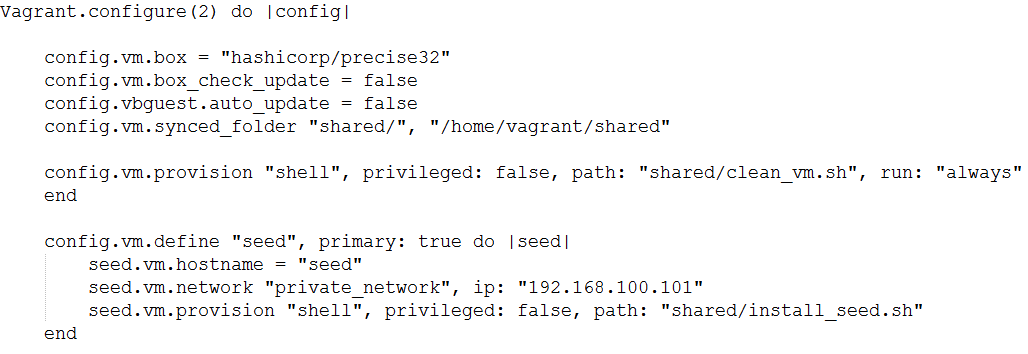
\includegraphics[width=140mm, keepaspectratio]{figures/vagrantfile.png}
	\caption{Egy Vagrantfile tartalma (részlet)}
	\label{fig:vagrantfile}
\end{figure}

\Aref{fig:vmcreate}-es ábra egy virtuális gép létrehozásának folyamatát ábrázolja mind a Vagrant által létrehozott, mind a mi általunk manuálisan készített VM esetére.

\begin{figure}[ht]
	\centering
	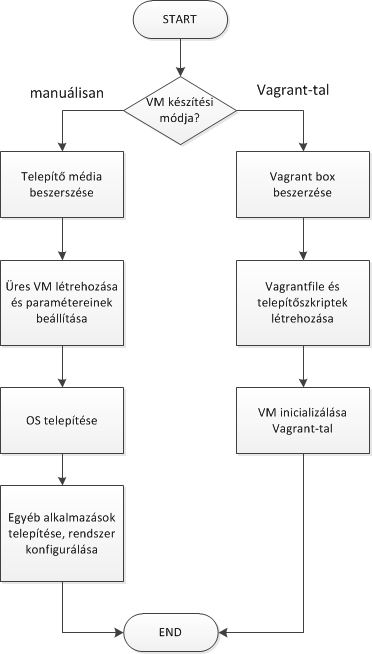
\includegraphics[height=140mm, keepaspectratio]{figures/vmcreate.png}
	\caption{Virtuális gép létrehozásának a folyamata}
	\label{fig:vmcreate}
\end{figure}

Egy virtuális gép reprezentálásához a gazdagépen alapvetően háromféle fájl szükséges legalább:

\begin{itemize}
	\item Egyik a futtatásához szükséges konfigurációs beállításokat írja le (VM metaadatai, szükséges erőforrások stb.).
	\item Másik a VM által használt virtuális lemezeken található adatokat tartalmazza.
	\item Opcionálisan lehetnek úgynevezett snapshot-ok is, amelyek egy konkrét állapotát írják a virtuális gépnek, ahova bármikor visszaállítható.
\end{itemize}

Ezeket a fájlokat terítjük a laborban.
%----------------------------------------------------------------------------
\section{Peer-to-peer fájlátvitel} 
\label{sect:p2p}
%----------------------------------------------------------------------------
A Peer-to-Peer(P2P) hálózat olyan, aminek a csomópontjai nem egy kitüntetett géppel 
kommunikálnak, hanem közvetlenül egymással. A klasszikus kliens-szerver és a P2P hálózat felépítését
\aref{fig:networkcomparison}-as ábra szemlélteti.

\begin{figure}[ht]
	\centering
	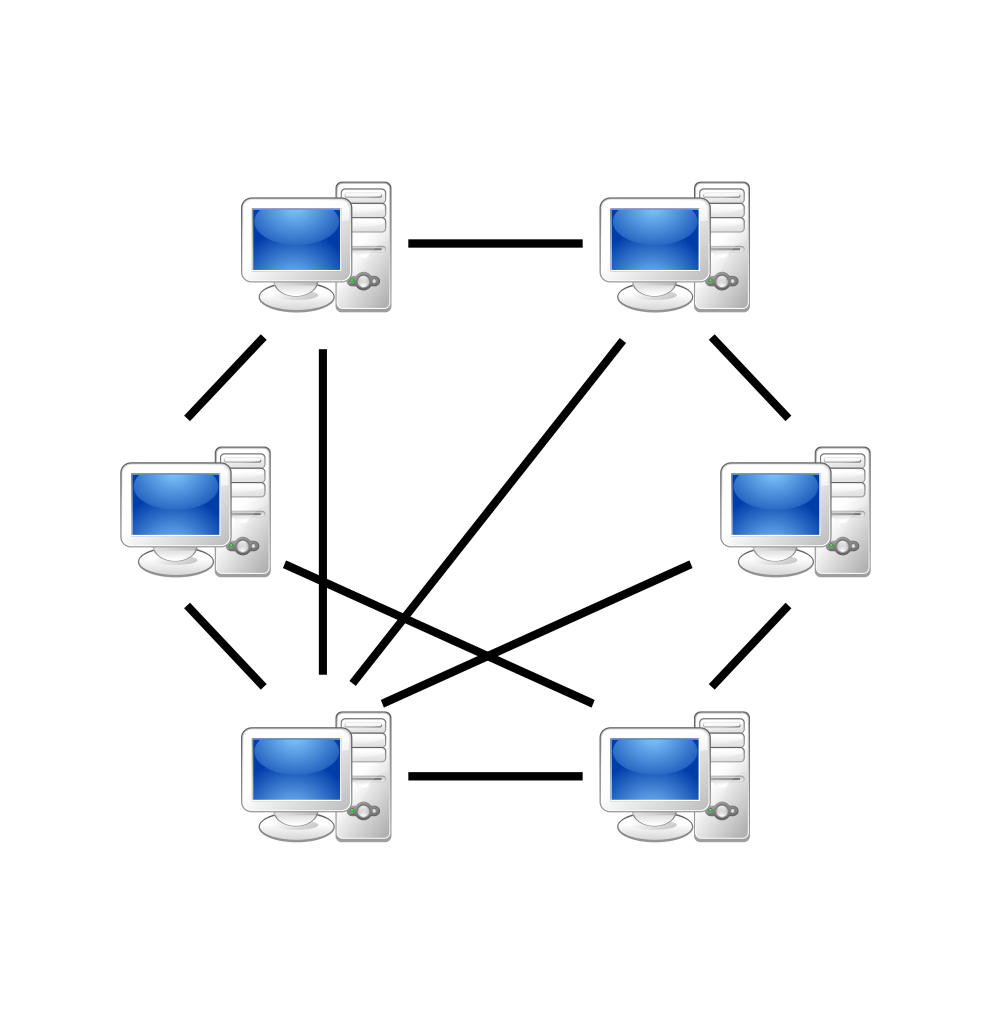
\includegraphics[width=50mm, keepaspectratio]{figures/P2P-network.png}\hspace{1cm}
	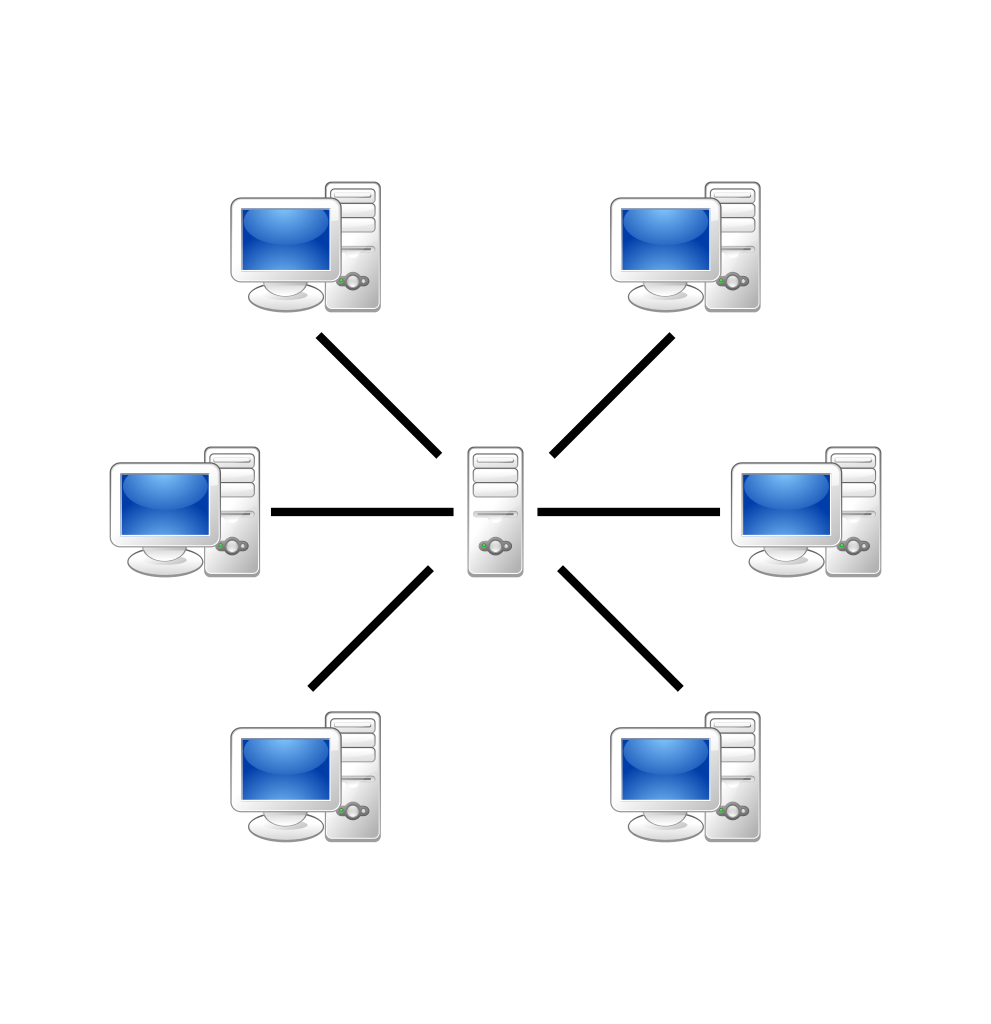
\includegraphics[width=50mm, keepaspectratio]{figures/Server-based-network.png}
	\caption{P2P és kliens-szerver alapú hálózat. \\(\textit{forrás: https://en.wikipedia.org/wiki/Peer-to-peer})}
	\label{fig:networkcomparison}
\end{figure}

P2P hálózat használatának fő előnye a robusztusság és a skálázhatóság, mivel nincs központi elem,
aminek a meghibásodása szolgáltatáskiesést okozhatna, illetve a hálózat min (például P2P alapú fájlmegosztás esetén a letöltés mellett fel is tölt). Hátrányai közül a két legjelentősebb a nehezebb karbantarthatóság és az internetszolgáltató-oldali forgalomkorlátozások miatt fellépő sebességproblémák.

A P2P alapú technológiák egyik legnagyobb felhasználási területe a tartalomszolgáltatás, ezen belül
az egyik legismertebb ilyen technológiát használó protokoll a Bittorrent. A Bittorrent~\cite{cohen2008bittorrent} protokollt
fájlmegosztásra használjuk, a mögötte álló alapvető ötlet az, hogy a megosztandó fájlokat
feldaraboljuk, és a letöltőknek ezeket a darabokat nem ugyanolyan sorrendben adjuk oda, így ők a
hiányzó darabokat egymástól is tudják tölteni. Ahhoz, hogy a letöltők megtalálják egymást, illetve a kész fájlt feltöltőket, az ún. \textbf{tracker} segít, ami adott átvitel résztvevőinek (a ``\textbf{swarm}'') adatainak tárolásáért felel. A Bittorrent terminológiájában a teljes fájlal rendelkező, már csak feltöltést végzőket \textbf{seed}-nek, a letöltőket, akik persze fel is töltenek \textbf{leecher}-nek vagy peer-nek nevezik. A tracker kiesése esetén léteznek más módszerek is a többi swarm-tag megtalálására, többek között a DHT\cite{rescorla2006introduction}(distributed hash table - elosztott hashtábla) használata, viszont esetünkben ez nem opció, mert az egyetem szabályzata tiltja a Bittorrent protokoll használatát (legalábbis a ``nagyvilág'' felé), a DHT bekapcsolása esetén pedig nem tudjuk a laborgépeinken futó torrentkliensek közti forgalmat a helyi hálóra izolálni.

Látszik, hogy torrent alapú fájlátvitel megvalósításához legkevesebb ezekre lesz szükségünk:
\begin{itemize}
	\item Minden laborgépen egy torrentkliensre
	\item Saját torrent tracker-re
	\item Seed gép kijelölésére
	\item Egy olyan programra, ami ezek működését vezérli
\end{itemize}
Az itt felsorolt elemekből felépülő terítési megoldás leírásához lásd majd \aref{design_apparchi}-as fejezetet. 

Gépeinkre telepítendő torrentkliens esetében az rtorrent-re\cite{sundell2012libtorrent} esett a választás, mivel szükségünk van arra, hogy olyan klienst használjunk, amit a háttérben is tudunk futtatni, illetve az állapota valami módon távolról is lekérhető legyen. Az rtorrent rendelkezik egy XMLRPC\cite{merrick2006xml} alapú interfésszel, aminek segítségével távolról is vezérelhetővé válik. Ilyen interfészt használ a számos rtorrent-hez írt webes felület is, például a legismertebb ruTorrent\cite{rutorrent}. Természetesen minden rtorrent-et futtató gépre telepítenünk kell egy webszervert is, ami az XMLRPC kéréseinket eljuttatja magának a torrentkliensnek, itt a választás az apache-ra\cite{fielding1997apache} esett főleg könnyű telepítése és konfigurálása miatt.

Tracker-ből az opentracker nevű került fel egy gépre (az egyszerűség kedvéért arra, amelyiket a terítések során seed-nek fogunk használni). Választásunk rá azért esett, mert különösebb funkcionális különbség nincs a lehetséges jelöltek között, ezt viszont könnyen lehet telepíteni a laborgépeken futó operációs rendszer csomagkezelőjéből. Amiről még eddig nem esett szó, az a protokoll működéséhez szükséges, metaadatokat tartalmazó fájl, a torrentfájl. Ez tárolja az adott letöltéshez tartozó fájlok hash-eit, amik adott fájl tartalmából előállított egyedi hexadecimális számok, tulajdonságuk, hogy ugyanarra a fájlra mindig ugyanaz a szám áll elő, másikra pedig szinte biztosan különböző, ezek alapján tudjuk ellenőrizni a letöltött adatok hibamentességét. A torrent fájl tartalmazza még ezen kívül a küldendő fájlok mappastruktúráját, metaadatait (pl. fájlnév, fájlméret) és a tracker címét. A torrentkliens és a tracker egy torrentfájlra az infohash alapján hivatkozik, ami a torrentfájl hash-ének kódolásával kapható meg, erre nekünk később akkor lesz szükségünk, amikor majd a terítés közben annak állapotának lekérésekor hivatkozni akarunk egy átvitelre.

Torrentfájlok létrehozására az mktorrent-et\cite{mktorrent} fogjuk használni.

\Aref{fig:torrentflow}-es ábrán egy fájl torrent alapú terítésének a folyamatát illusztrálja, onnan kezdve, hogy a fájl már a seed gépre van másolva odáig, hogy elkezdődik a célgépek által a fájl letöltése.

\begin{figure}[ht]
	\centering
	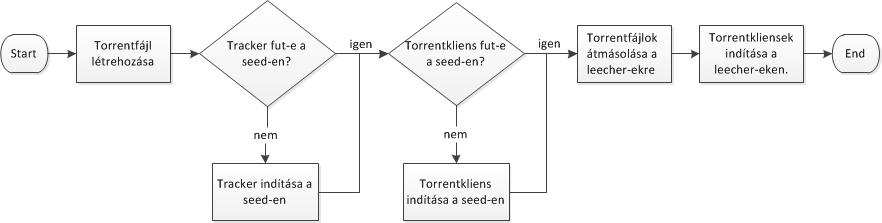
\includegraphics[width=150mm, keepaspectratio]{figures/torrentflow.png}
	\caption{Egy fájl torrent alapú terítésének folyamata.}
	\label{fig:torrentflow}
\end{figure}


%----------------------------------------------------------------------------
\section{Metamodellezés}
%----------------------------------------------------------------------------
Egy fájlterítés indításához két dologra van szükségünk, hogy mit és hova szeretnénk teríteni. Előző kérdésre \aref{sect:p2p}-es fejezet választ adott, az utóbbira ez fog. A ``hovának'' megadását sokféleképpen elképzelhetjük,  felhasználói szemszögből az lenne a legjobb, ha egyszerűen azt mondhatnánk, hogy ``az IB413-as laborban a Mérés Labor 4. tárgyhoz tartozó környezet terüljön.'' Fontos, hogy képes legyen az alkalmazás egy ilyen kérést végrehajtani, ha a kérést számára értelmezhetőbb formában adjuk át. 
A virtuális gép terítési feladatokat érdemes egy saját, úgynevezett szakterület-specifikus nyelven modellezni (angolul Domain-Specific Language, DSE). Egy szakterület-specifikus nyelv legfőbb koncepcióit, kapcsolatait és alapvető struktúráját határozza meg a metamodell. Például egy labor metamodellje alatt egy olyan nyelvet kell elképzelni, amiben leírható tetszőleges oktatási labor. \Aref{fig:emfobj}-ös ábra egy ilyen metamodell egyik osztályát ábrázolja.

\begin{figure}[ht]
	\centering
	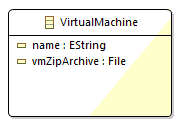
\includegraphics[width=50mm, keepaspectratio]{figures/binf_emf_1.png}
	\caption{Metamodell osztály - \textit{Terítendő virtuális gépeket ábrázolja, lehetséges attribútumai a VM neve és a hozzá tartozó fájlokat tároló tömörített állomány elérési útvonala.}}
	\label{fig:emfobj}
\end{figure}

Metamodell osztályok között lehetnek kapcsolatok is, amelyek közül a két legfontosabb a tartalmazás(kompozíció) és a referencia. \Aref{fig:emfcomp}-os ábrán egy kompozícióra, \ref{fig:emfref}-esen egy referenciára láthatunk példát.

\begin{figure}[ht!]
	\centering
	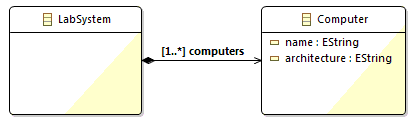
\includegraphics[width=115mm, keepaspectratio]{figures/binf_emf_2.png}
	\caption{Kompozíció - \textit{Azt írja le, hogy a laborunk tetszőleges számú (minimum 1 darab) számítógépből áll.}}
	\label{fig:emfcomp}
\end{figure}

\begin{figure}[ht!]
	\centering
	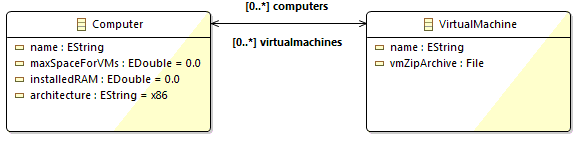
\includegraphics[width=150mm, keepaspectratio]{figures/binf_emf_3.png}
	\caption{Referencia - \textit{Egy számítógépen tetszőleges VM lehet, illetve egy VM tetszőleges számú számítógépen lehet rajta.}}
	\label{fig:emfref}
\end{figure}


Egy ilyen metamodell segítségével létrehozhatunk egy, a laborok leírására alkalmas modellezési nyelvet, ennek a gyakorlati használatát segíti az Eclipse Modeling Framework\cite{steinberg2008emf}. Az EMF-el az elkészített metamodell használatát tudjuk Java programokba integrálni, továbbá szerkesztőfelületet is létre tud hozni adott modell adatainak kitöltéséhez. Az EMF által, a metamodellből generált forráskódot használva a programunk egyszerűen be tud tölteni modellfájlokat, így tehát a terítést tudjuk vezérelni az EMF-ben létrehozott modellel, ami leírja a labor felépítését és a terítés célállapotát.